% $Id: TimeMgr_obj3.tex,v 1.1 2002/08/18 22:43:36 eschwab Exp $

%\section{Object Model}

Whereas Figures 1 and 2 are static structure UML diagrams, Figures 3, 4,  and
5 are dynamic behavioral UML diagrams.  Figure 3 shows how timestepping occurs
within an instance of Time Manager.  First, an ESM component invokes the
Advance() method on its clock, named ModelTime in this example.  In turn,
ModelTime increments its internal current time TimeInstant, called CurrTime.
A user only needs to know how to create a clock and invoke its Advance()
method.  The implementation detail of actually performing the increment is
hidden from the user as it is encapsulated within the Time Manager clock.

\begin{center}
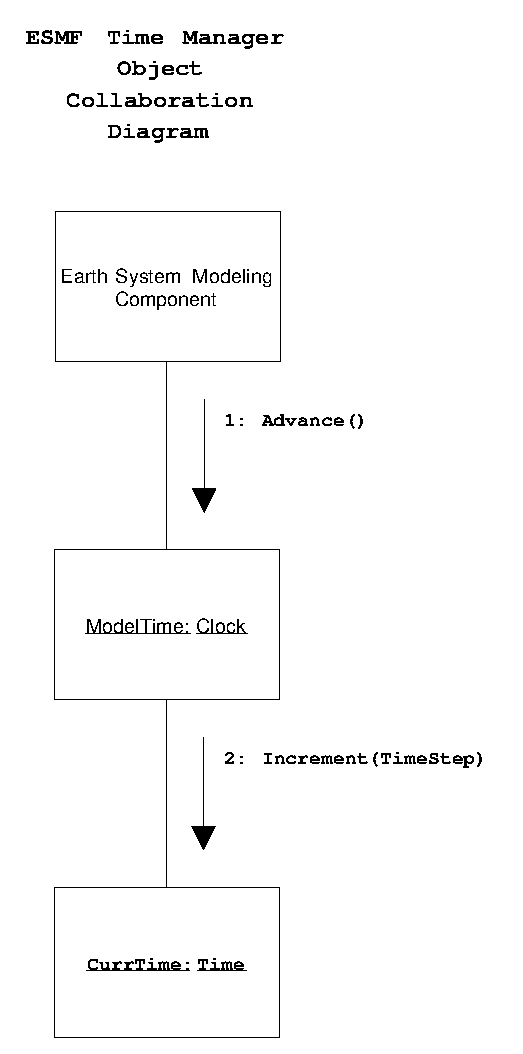
\includegraphics{TimeMgrOCD1.EPS}
   
Figure 3.  ESMF Time Manager Increment Model Time Scenario
   
\end{center}
